%%%%%%%%%%%%%%% COPYRIGHT ANTOINE HUGOUNET & ETHEL VILLENEUVE
%%%%%%%%%%%%%%%%%%%%%%%%%%%%%%%%%%%%%%%%%%%%%%%%%%%%%%%
%%%%%%%%%%%%%%%%%%%%%%%%%%%%%%%%%%%%%%%%%%%%%%%%%%%%%%%


\documentclass[a4paper, twoside, 11pt]{report}

\usepackage[utf8]{inputenc}
\usepackage[T1]{fontenc}
\usepackage[english]{babel}
\usepackage[top= 120pt, left=80pt, right=80pt]{geometry} %marges
\usepackage{setspace} %interlignage
\usepackage{url}
\usepackage{graphicx}
\usepackage{lmodern} 
\usepackage{array}
\usepackage{csquotes}
\usepackage[numbers,square]{natbib}
\usepackage{soul}
\usepackage{hyperref}
\usepackage{amsthm}
\usepackage{color}
\usepackage[usenames,dvipsnames,svgnames,table]{xcolor}
\usepackage{adjustbox}
\usepackage{amssymb}
\usepackage{amsmath}
\usepackage{dsfont}
%%\usepackage{braket}
\usepackage{physics}
\usepackage{amsfonts}
\usepackage[numbers,square]{natbib}
\usepackage{multirow}
\usepackage{listings}
\usepackage{wasysym}

%%%%%% COULEURS CODE C++
\lstdefinestyle{customc}{
  belowcaptionskip=1\baselineskip,
  breaklines=true,
  frame=L,
  xleftmargin=\parindent,
  language=C,
  showstringspaces=false,
  basicstyle=\footnotesize\ttfamily,
  keywordstyle=\bfseries\color{red},
  commentstyle=\itshape\color{gray},
  identifierstyle=\color{NavyBlue},
  stringstyle=\color{black},
}

\lstdefinestyle{customasm}{
  belowcaptionskip=1\baselineskip,
  frame=L,
  xleftmargin=\parindent,
  language=[x86masm]Assembler,
  basicstyle=\footnotesize\ttfamily,
  commentstyle=\itshape\color{purple!40!black},
}

\lstset{escapechar=@,style=customc}

%%%%%% STYLES DE THÉORÈMES

\newtheoremstyle{theorem}%	Name
  {}%	Space above
  {}%	Space below
  {}%	Body font
  {}%	Indent amount
  {\bfseries}%	Theorem head font
  {.}%	Punctuation after theorem head
  { }%	Space after theorem head, ' ', or \newline
  {}%	Theorem head spec (can be left empty, meaning `normal')

\newtheoremstyle{exemple}%	Name
  {}%	Space above
  {}%	Space below
  {\color{Gray}\itshape}%	Body font
  {}%	Indent amount
  {\color{Gray}\itshape}%	Theorem head font
  {.}%	Punctuation after theorem head
  { }%	Space after theorem head, ' ', or \newline
  {}%	Theorem head spec (can be left empty, meaning `normal')

\newtheoremstyle{remark}%	Name
  {}%	Space above
  {}%	Space below
  {\itshape}%	Body font
  {}%	Indent amount
  {\bfseries}%	Theorem head font
  {.}%	Punctuation after theorem head
  { }%	Space after theorem head, ' ', or \newline
  {}%	Theorem head spec (can be left empty, meaning `normal')
  
%%%%%% DÉCLARATION DES THÉORÈMES

\theoremstyle{theorem}
\newtheorem{theorem}{Theorem}[section]
\newtheorem{lemme}{Lemma}[section]
\newtheorem{proposition}{Proposition}[section]
\newtheorem{definition}{Definition}[section]

\theoremstyle{remark}
\newtheorem{remark}{Remark}[chapter]

\theoremstyle{exemple}
\newtheorem*{exemple}{Example}


%%%%%% COMMANDES QUI SIMPLIFIENT LA VIE

\newcommand{\legende}[1]{
\begin{center}
	\begin{minipage}{12cm}
		\begin{center}
			\textit{\textcolor{WildStrawberry!30}{#1}}
		\end{center}
	\end{minipage}
\end{center}}

\newcommand{\sherlock}[2]{
	\begin{equation}
		\textcolor{WildStrawberry}{#1}
	\end{equation}
	\legende{#2}
}
	
\newcommand{\sherlocked}[1]{
	\begin{equation}
		\textcolor{WildStrawberry}{#1}
	\end{equation}
}

	
\newcommand{\defSherlock}[3]{
	\begin{definition}[\textbf{#1}]
		\sherlock{#2}{#3}
	\end{definition}
}

\newcommand{\defSherlocked}[2]{
	\begin{definition}[\textbf{#1}]
		\sherlocked{#2}
	\end{definition}
}	

\newcommand{\propSherlock}[3]{
	\begin{proposition}[\textbf{#1}]
		\sherlock{#2}{#3}
	\end{proposition}
}

\newcommand{\propSherlocked}[2]{
	\begin{proposition}[\textbf{#1}]
		\sherlocked{#2}
	\end{proposition}
}

\newcommand{\textSherlocked}[1]{
	\begin{center}
		\textcolor{WildStrawberry}{#1}
	\end{center}
}

\newcommand{\N}{\mathbb{N}}
\newcommand{\Z}{\mathbb{Z}}
\newcommand{\R}{\mathbb{R}}
\newcommand{\C}{\mathbb{C}}


%%%%%%%%%%%%%%%%%%%%%%%%%%%%%%%%%%%%%%%%%%%%%%%%%%%%%%%
%%%%%%%%%%%%%%%%%%%%%%%%%%%%%%%%%%%%%%%%%%%%%%%%%%%%%%%
%%%%%%%%%%%%%%%%%%%%%%%%%%%%%%%%%%%%%%%%%%%%%%%%%%%%%%%

\title{FYS3150\\Project 3 - }
\author{Hugounet, Antoine \& Villeneuve, Ethel}
\date{September 2017 \\University of Oslo \\ \url{https://github.com/kryzar/Perseids.git}}



\begin{document}
\selectlanguage{english}
\maketitle
	
	
\begin{abstract}

	\paragraph{}
	
\end{abstract}


\tableofcontents


\chapter*{Introduction}
\addcontentsline{toc}{chapter}{Introduction}

    \paragraph{}
    

\chapter{Theory}
    
    \paragraph{}In a first place, we will begin with an Earth-Sun system with the Earth orbiting around the Sun to test a simple algorithm and then we will add the other planets to have a simulation of the complete Solar System. 

    \section{Earth-Sun system}
        \subsection{Physical conditions of the system}
            \paragraph{}The only force applied to this system is the gravity. According to the Newton's law, we have 
                \begin{equation*}
                F_G = \frac{GM_{\odot}M_{\oplus}}{r^2}
                \end{equation*}
            with $F_G$ the gravitational force, $G$ the gravitational constant ($G=6.674 \times 10^{-11} \mathrm{N}.\mathrm{m}^2.\mathrm{kg}^{-2}$), $M_{\odot}$ the mass of the Sun, $M_{\oplus}$ the mass of the Earth and $r$ the distance between the Earth and the Sun.\\
            We will neglect the motion of the Sun here as the mass of the Sun is much larger than the mass of the Earth ($M_{\odot} = 2 \times 10^{30}$kg against $M_{\oplus} = 6 \times 10^{24}$kg). We want to establish the motion of the Earth around the Sun. Moreover, we will assume that the orbit of the Earth around the Sun is coplanar in the $xy$-plane.
            \paragraph{}The Newton's second law of motion is given by $F=M \times a$ with $F$ the force applied to the system, $M$ the mass of the body concerned and $a$ the acceleration. Applied to our case, we have $F_G = M_{\oplus} \times a$, $a$ being the second derivative of the position, which can be written in two equations : 
                \begin{align*}
                    F_{G,x} &= M_{\oplus} \frac{d^2 x}{dt^2} \\
                    F_{G,y} &= M_{\oplus} \frac{d^2 y}{dt^2}
                \end{align*}
            or
                \begin{align}
                    \frac{d^2 x}{dt^2} &= \frac{F_{G,x}}{M_{\oplus}} \tag{1}\\
                    \frac{d^2 y}{dt^2} &= \frac{F_{G,y}}{M_{\oplus}} \tag{2}.
                \end{align}
            with $F_{G,x}$ and $F_{G,y}$ the components of the gravitational force.\\
            We will not use the SI units but the Astronomical units (AU) for the distances (with $1$AU$=$average distance Earth-Sun $=1.5 \times 10^{11}$m), kg for masses and years for time units. \\
            In this case, the initial position of the Earth will be $x_{\oplus} = 1$, \hspace{0,1cm}$y_{\oplus} = 0$ with the Sun the origin ($x_{\odot} = 0$, $y_{\odot} = 0$). \\
            To simplify a little bit, we will assume that the Earth's orbit is circular around the Sun. So we can write :
                \begin{equation}
                    F_G = \frac{M_{\oplus} v^2}{r} = \frac{GM_{\odot}M_{\oplus}}{r^2}
                    \tag{3}
                \end{equation}
            with $v$ the velocity of Earth. From here we have
                \begin{equation*}
                    v^2 r = GM_{\odot} = 4 \pi^2 \mathrm{AU}^3 / \mathrm{yr}^2
                    \tag{4}
                \end{equation*}
            
        \subsection{Escape velocity}
            \paragraph{}In the case where only the gravitational force is applied, the mechanical energy $E_m = E_c + E_p$ with $E_c$ the kinetic energy and $E_p$ the potential energy is conserved as the gravitational force is conservative. For a planet at a distance of 1 AU from the Sun (let's take the Earth as an example), the kinetic energy is given by $E_c = \frac{1}{2}M_{\oplus}\times v^2$ and the potential energy by $E_p = - \frac{G M_{\odot} M_{\oplus}}{r}$ with $r=1$ AU.\\ 
            We want this planet to escape from the gravitational attraction of the Sun on it. The escape velocity will be the minimal speed $v_e$ at which the planet escapes from the gravitational influence of the Sun. We consider two positions of the planet : $p_i$ the initial position when $r_i=1$AU and $p_f$ the final position when the planet has escaped and is at an infinite distance from the Sun $r_f=\infty$. Let's consider the mechanical energy at the final position. We have $E_{m_f} = E_{c_f} + E_{p_f}$, $E_{c_f} = 0$ as the velocity of the planet is zero at the final state, $E_{p_f}=0$ as the planet has escaped from the gravitational attraction of the Sun. $E_{m_f}=0$. \\
            So, with the planet at 1 AU from the Sun at its inital position, of which velocity is the escape velocity $v_e$, in the case where there is only the gravitational force applied to the system planet-Sun, we have :
                \begin{equation*}
                    E_{c_i} + E_{p_i} = \frac{1}{2}M_{\oplus} \times v_e^2 - \frac{GM_{\odot}M_{\oplus}}{r_i} = E_{c_f} + E_{p_f} = 0
                \end{equation*}
            according to the law of conservation of energy. From this we can write
                \begin{align*}
                    \frac{1}{2}M_{\oplus} \times v_e^2 &- \frac{GM_{\odot}M_{\oplus}}{r_i} = 0 \\
                    \Rightarrow v_e &= \sqrt{\frac{2GM_{\odot}}{r_i}} \\
                    \Rightarrow v_e &=\sqrt{2GM_{\odot}}
                \end{align*}
            which only depends on the mass of the Sun. 
                \begin{align*}
                    v_e &= \sqrt{2\times 4\pi^2}, \hspace{0.5cm} \mathrm{from (4)}\\
                    v_e &= 2\sqrt{2}\pi \hspace{0.2cm} \mathrm{AU/yr}
                \end{align*}
            Then, for a velocity $v \geq 2\sqrt{2}\pi$, the Earth would escape from the Sun's gravitational attraction. 
                        
                        
    
    \section{Three-body problem}
        \paragraph{}We add Jupiter to the previous system.
        
        \subsection{The Sun as the center-of-mass}
            \paragraph{}In the previous case, the Earth's motion had a stable circular orbit in time. Adding Jupiter, the Earth's motion will inevitably be disturbed. We can write the gravitational between the Earth and Jupiter as 
                \begin{equation*}
                    F_{\oplus-\jupiter} = \frac{GM_{\jupiter}M_{\oplus}}{r_{\oplus-\jupiter}^2} 
                \end{equation*}
            with $M_{\jupiter}$ the mass of Jupiter and $r_{\oplus - \jupiter}$ the distance between the Earth and Jupiter. \\
            The algorithm used for this case will be exactly the same as the previous case. We will see in section 1.4 how to discretize and implement the algorithm. 
            
        \subsection{Real center-of-mass}
            \paragraph{}To get closer to the reality, we now do not consider the Sun as a static body anymore. Each of three bodies are in motion. Moreover, the center-of-mass will not be the Sun but the real one. Let's compute the center-of-mass coordinates.
                \begin{align*}
                    x_c &= \frac{1}{M_{tot}}\sum\limits_{i} M_i x_i\\
                    y_c &= \frac{1}{M_{tot}}\sum\limits_{i} M_i y_i
                \end{align*}
            We consider the system Earth-Jupiter-Sun.
                \begin{align*}
                    M_{tot} &= M_{\oplus} + M_{\jupiter} + M_{\odot} \\
                    M_{tot} &= 6\times10^{24} + 1.9\times 10^{27} + 2 \times 10^{30}\\
                    M_{tot} &= 2.00191 \times 10^{30} \mathrm{kg}
                \end{align*}
                \begin{equation*}
                    \left\{
                        \begin{aligned}
                            x_c = \frac{1}{M_{tot}} [M_{\oplus} x_{\oplus_i} + M_{\jupiter} x_{\jupiter_i} + M_{\odot} x_{\odot_i}] \\
                            y_c = \frac{1}{M_{tot}} [M_{\oplus} y_{\oplus_i} + M_{\jupiter} y_{\jupiter_i} + M_{\odot} y_{\odot_i}]
                        \end{aligned}
                    \right.
                \end{equation*} 
            We fix the initial positions with respect to the new center of mass. We want the three bodies and the center-of-mass aligned like that :
            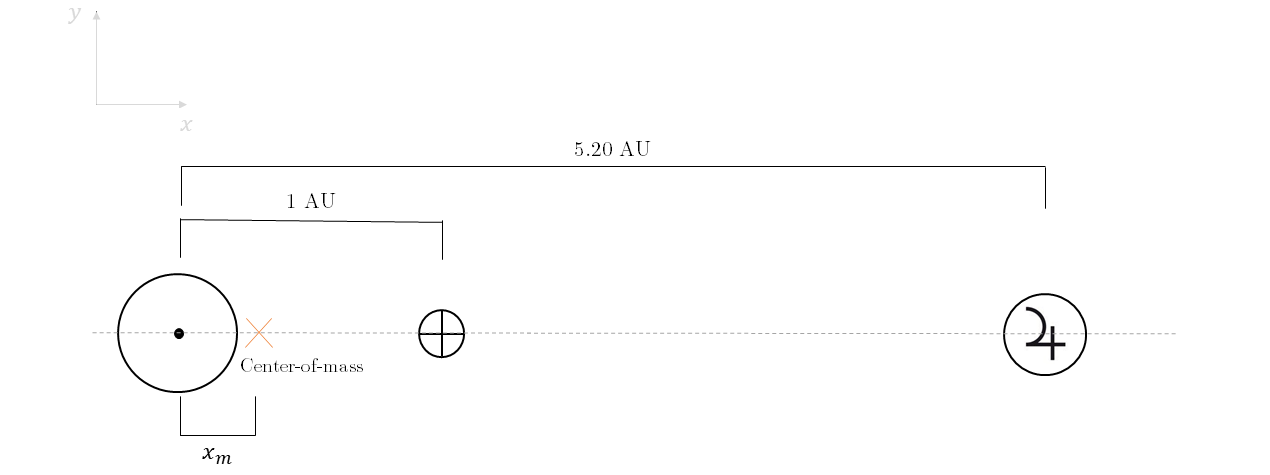
\includegraphics{dessinplanete.png}
            So we look for the $x_m$ so that $x_c$ and $y_c$ are equal to zero.
                \begin{equation*}
                    \left\{
                        \begin{aligned}
                            x_c &= \frac{1}{2.00191 \times 10^{30}} [(2 \times 10^{24}) \times (1 + x_m) + (1.9 \times 10^{27}) \times (5.20 + x_m) + (2 \times 10^{30}) \times x_m] = 0 \\
                            y_c &= 0 
                        \end{aligned}
                    \right.
                \end{equation*}
                \begin{equation*}
                    \left\{
                        \begin{aligned}
                            \frac{1}{2.00191\times 10^{30}}[x_m (2\times10^{24} + 1.9\times10^{27} + 2\times 10^{30}) + (2\times10^{24} + 5.20 \times 1.9 \times 10^{27} = 0 \\
                            y_m = 0
                        \end{aligned}
                    \right.
                \end{equation*}
                \begin{equation*}
                    \left\{
                        \begin{aligned}
                            x_m &= -\frac{2\times 10^{24} + 5.20 \times 1.9 \times 10^{27}}{M_{tot}}\\
                            y_m &= 0
                        \end{aligned}
                    \right.
                \end{equation*}
                \begin{equation*}
                    \left\{
                        \begin{aligned}
                            x_m &= -4.936 \times 10^{-3}\\
                            y_m &= 0
                        \end{aligned}
                    \right.
                    \tag{5}
                \end{equation*}
            These are the coordinates of the Sun when the center-of-mass of the system is set as the origin. Let's now compute the Sun's initial velocity so that the total momentum of the three-body system would be equal to zero.
                \begin{align*}
                    \vec{p_{tot}} &= \sum\limits_{k} M_k \vec{k} \\
                    \left(\begin{array}{c}
                            0\\
                            0
                    \end{array} \right) &= M_{\oplus} 
                        \left(\begin{array}{c}
                                v_{\oplus_x}\\
                                v_{\oplus_y}
                        \end{array} \right) + M_{\jupiter}
                             \left(\begin{array}{c}
                                    v_{\jupiter_x}\\
                                    v_{\jupiter_y}
                            \end{array} \right) + M_{\odot}
                                \left(\begin{array}{c}
                                        v_x\\
                                        v_y    
                                \end{array} \right)
                \end{align*}
                \begin{equation*}
                    \left\{
                        \begin{aligned}
                            M_{\oplus} v_{\oplus_x} + M_{\jupiter} v_{\jupiter_x} + M_{\odot} v_x = 0 \\
                            M_{\oplus} v_{\oplus_y} + M_{\jupiter} v_{\jupiter_y} + M_{\odot} v_y = 0
                        \end{aligned}
                    \right.
                \end{equation*}
            We take the initial velocities of the Earth and Jupiter so that their orbit will be circular.\\
            If the orbit of the Earth is circular, $v_{\oplus} = 2 \pi $ AU/yr, because the distance travelled in one Earth-year is $2 \pi \times r$ with $r = 1$ AU. The velocity is constant so the initial velocity will be $v_{\oplus_i}=2\pi$ AU/yr. In the initial configuration represented above, the initial velocity is oriented in the direction of $y$. So, $v_{\oplus_i} = \left(\begin{array}{c}
                0\\
                2 \pi
            \end{array} \right)$ \\
            Jupiter has an orbital period of $11.862$yr. The distance travelled by Jupiter in this period is $2 \pi \times r = 2 \pi \times 5.20 = 32.673 AU$. So $v_{\jupiter_i}= \frac{2 \pi \times r}{T} = \frac{2 \pi \times 5.20}{11.862} = 2.7544 $ AU/yr. Similarly, the initial velocity can be expressed as $v_{\jupiter_i} = \left(\begin{array}{c}
                0 \\
                2.7544
                \end{array} \right)$ 
                \begin{equation*}
                    \left\{
                        \begin{aligned}
                            &(6\times 10^{24}) \times 0 + (1.9 \times 10^{27}) \times 0 + (2 \times 10^{30}) \times v_x = 0 \\
                            &(6\times 10^{24}) \times 2 \pi + (1.9 \times 10^{27}) \times 2.7544 + (2 \times 10^{30}) \times v_y = 0
                        \end{aligned}
                    \right.
                \end{equation*}
                \begin{equation*}
                    \left\{
                        \begin{aligned}
                            v_x &= 0\\
                            v_y &= - \frac{(6\times 10^{24}) \times 2 \pi + (1.9 \times 10^{27}) \times 2.7544}{2 \times 10^{30}}
                        \end{aligned}
                    \right.
                \end{equation*}
                \begin{equation*}
                    \left\{
                        \begin{aligned}
                            v_x &= 0\\
                            v_y &= 2.6355 \times 10^{-3}
                        \end{aligned}
                    \right.
                \end{equation*}
            To have a fixed center-of-mass, the Sun will need a velocity $v =
            \left(\begin{array}{c}
                0\\
               2.6355 \times 10^{-3}
            \end{array} \right)$.                
    

    \section{The complete Solar system}
        \paragraph{}
        

    \section{Discretization}
        \subsection{Euler's method}
            \paragraph{Acceleration.}To implement the accelerations, we normalize the masses with respect to the mass of the Sun. Thus, $M_{\odot}=1$, $M_{k_N}=\frac{M_k}{M_{\odot}}$ is the normalized mass for each body $k$.
            \paragraph{} From the Newton's law of motion, the acceleration of a given body can be written as $a=\frac{F_G}{M}$, with $M$ the mass of the body. 
                \begin{equation*}
                    a_i = \frac{ \sum\limits_{k} \frac{GMM_{k_N}}{r_k^2}}{M}
                \end{equation*}
            with $k$ the number of bodies involved in the system. 
                \begin{equation*}
                    a_i = \sum\limits_{k} \frac{GM_{k_N}}{r_k^2}
                \end{equation*}
            From (4), we have $GM_{\odot} = 4\pi^2\mathrm{AU}^3/\mathrm{yr}^2$ and as $M_{\odot}=1$, $G=4\pi^2\mathrm{AU}^3/\mathrm{yr}^2$. So,
                \begin{align*}
                    a_i &= \sum\limits_{k} \frac{4\pi^2M_{k_N}}{r_k^2} \\
                    a_i &= \sum\limits_{k} \frac{4\pi^2M_{k_N}(x_i-x_{i_k})}{r_k^3} 
                    \tag{7}
                 \end{align*}
             With Euler's method, we can write $\displaystyle a_i=\frac{v_{i+1} - v_i}{h}$ with $\displaystyle h = \frac{b-a}{N}$ the step length and $N$ the number of mesh points. Therefore, 
                \begin{align*}
                     &\frac{v_{i+1} - v_i}{h} = \sum\limits_{k}\frac{4\pi^2M_k(x_i-x_{i_k})}{r_k^3} \\
                     \Rightarrow &v_{i+1} = h\sum\limits_{k}\frac{4\pi^2M_k(x_i-x_{i_k})}{r_k^3} + v_i
                    \tag{8}
                \end{align*}
             \paragraph{Velocity.}The velocity can easily be discretized as
                \begin{equation*}
                      v_i = \frac{x_{i+1}-x_i}{h}
                  \end{equation*}
             Therefore,
                 \begin{equation*}
                    x_{i+1} = hv_i + x_i
                    \tag{9}
                \end{equation*}   
            The initial position and velocity of the body are obtained with the data from the NASA website.
            
        \subsection{Verlet's method}
            \paragraph{}The Verlets method is almost the same as the Euler's one but is more precise. It is based on a Taylor expansion of the position. We consider two instants $t_i+h$ as $t_i-h$ :
                \begin{equation*}
                    \left\{ 
                        \begin{aligned}
                            x_{i+1} &= x(t_i+h) = x(t_i) + h\frac{dx}{dt}(t_i) + \frac{h^2}{2!}\frac{d^2x}{dt^2}(t_i) + \frac{h^3}{3!}\frac{d^3x}{dt^3}(t_i)+\mathcal{O}(h^4)\\
                            x_{i-1} &= x(t_i-h) = x(t_i) - h\frac{dx}{dt}(t_i) + \frac{h^2}{2!}\frac{d^2x}{dt^2}(t_i) - \frac{h^3}{3!}\frac{d^3x}{dt^3}(t_i)+\mathcal{O}(h^4)
                        \end{aligned}
                    \right.
                \end{equation*}
            We sum up the two lines to have
                \begin{align*}
                    x_{i+1} &+ x_{i-1} = 2x_i + h^2\frac{d^2x_i}{dt^2} + \mathcal{O}(h^4) \\
                    \Rightarrow x_{i+1} &= 2x_i - x_{i-1} + h^2\frac{d^2x_i}{dt^2} + \mathcal{O}(h^4)
                \end{align*}
            


\chapter{Implementation}

    \section{Earth-Sun system}
        \subsection{}
        
        \subsection{Tests}
            \paragraph{}The mechanical energy $E_m = E_c + E_p$ should be conserved because the only force taken into account is the gravitational force, which is conservative. The potential energy is constant in time ($E_p = -\frac{GM_{\oplus}M_{\odot}}{r} \forall t$), so is conserved. The kinetic energy depends on the velocity of the Earth ($E_c = \frac{1}{2}M_{\oplus}v^2$, which is constant in time as we have a uniform circular motion of the Earth around the Sun. So as both of the kinetic and potential energies are constant in time, for any $t_i$ and $t_f$ we have
                \begin{equation*}
                    \left\{
                        \begin{aligned}
                            E_{c_i} &= E_{p_f}\\
                            E_{p_i} &= E_{p_f}
                        \end{aligned}
                    \right. \hspace{0.5cm} \Rightarrow E_{c_i} + E_{p_i} = E_{c_f} + E_{p_f}
                \end{equation*} 
                \begin{equation*}
                    \Rightarrow E_{m_i} = E_{m_f}
                \end{equation*}
                        
    
    \section{Adding one planet}
    
    
    \section{The complete Solar system}
    
    

\chapter{Results}

    \section{Earth-Sun system}  
        \subsection{} 
    
    
    \section{Three-body problem}
        \subsection{The Sun as the center-of-mass}
        
        \subsection{The real center-of-mass}
    
    
    \section{Complete Solar System}
        \subsection{}
        
        \subsection{}
    
    

\chapter*{Conclusion}
\addcontentsline{toc}{chapter}{Conclusion}

    \paragraph{}
    
    
    
    
\chapter*{Bibliography}
    \begin{itemize}
        \item NASA website \href{{http://ssd.jpl.nasa.gov/horizons.cgi#top}}{\nolinkurl{http://ssd.jpl.nasa.gov/horizons.cgi\#top}}
        \item 
    \end{itemize}
    
    
    
    
    
    
    
    
    
    
\end{document}